% 05-unsupervised-learning-clustering.tex

% Unsupervised Learning – Clustering
% 5.1. Introduction: Provides an overview of the clustering task and its objectives.
% 5.2. Determine the Number of Clusters: Uses methods like the elbow method or silhouette analysis to determine the number of clusters.
% 5.3. Hyperparameter Tuning: Tunes other hyperparameters, if any.
% 5.4. Cluster Visualization: Visualizes the clusters through t-SNE.
% 5.5. Cluster Analysis: Analyzes the characteristics of each cluster.
% 5.6. Intent Homogeneity: Assesses if clusters reflect intent division.
% 5.7. Specific Attack Categories: Associates clusters with specific attack categories.

% Section Title
\section{UNSUPERVISED LEARNING - CLUSTERING}

    % Main Content

    \subsection{Introduction}
    
        This section provides an overview of the clustering task and its objectives. The goal is to group similar attack sessions into clusters based on their characteristics. By identifying clusters, we can gain insights into common patterns and behaviors in the attack data. We will use various clustering techniques and evaluate their effectiveness.

    \subsection{Determine the Number of Clusters}
    
        Determining the optimal number of clusters is a crucial step in the clustering process. We use methods like the elbow method and silhouette analysis to identify the appropriate number of clusters.

        \textbf{Elbow Method:} The elbow method involves plotting the sum of squared distances (inertia) for a range of cluster numbers and identifying the point where the inertia starts to decrease more slowly (the "elbow").
    
        \vspace{0.5em}

        \textbf{Refer to Appendix \ref{lst:elbow_method} for the code snippet.}

        \textbf{Figure \ref{fig:elbow-method}} shows the elbow method plot for k-Means clustering.

        \begin{figure}[h]
            \centering
            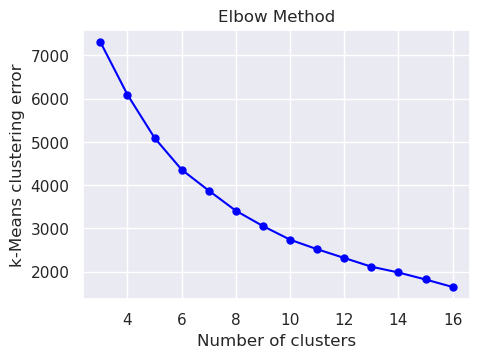
\includegraphics[width=0.8\textwidth]{../figures/plots/section3/k-means_clustering_error.png}
            \caption{Elbow Method for k-Means Clustering}
            \label{fig:elbow-method}
        \end{figure}

        \textbf{Silhouette Analysis:} Silhouette analysis involves calculating the silhouette score for each potential cluster number. The silhouette score measures how similar an object is to its own cluster compared to other clusters.
        
        \vspace{0.5em}

        \textbf{Refer to Appendix \ref{lst:silhouette_analysis} for the code snippet.}

        \textbf{Figure \ref{fig:silhouette-analysis}} shows the silhouette analysis plot for k-Means clustering.

        \begin{figure}[h]
            \centering
            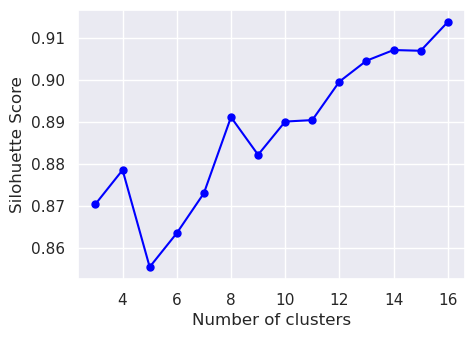
\includegraphics[width=0.8\textwidth]{../figures/plots/section3/k-means_silohuette_score.png}
            \caption{Silhouette Analysis for k-Means Clustering}
            \label{fig:silhouette-analysis}
        \end{figure}

        Based on the elbow method and silhouette analysis, we select the optimal number of clusters for further analysis.
            
    \subsection{Hyperparameter Tuning}
    
        Hyperparameter tuning involves optimizing the parameters of the clustering algorithms to improve their performance. We use GridSearchCV to perform an exhaustive search over specified parameter values.

        \textbf{K-Means Hyperparameter Tuning:}
    
        \vspace{0.5em}

        \textbf{Refer to Appendix \ref{lst:grid_search_kmeans} for the code snippet.}

        The best parameters for k-Means clustering were found to be:
        \begin{itemize}
            \item \textbf{init}: k-means++
            \item \textbf{n\_init}: 20
            \item \textbf{max\_iter}: 150
        \end{itemize}

        \textbf{Gaussian Mixture Model (GMM) Hyperparameter Tuning:}
        
        \vspace{0.5em}

        \textbf{Refer to Appendix \ref{lst:grid_search_gmm} for the code snippet.}

        The best parameters for GMM clustering were found to be:
        \begin{itemize}
            \item \textbf{init\_params}: kmeans
            \item \textbf{covariance\_type}: full
            \item \textbf{tol}: 1e-4
            \item \textbf{max\_iter}: 200
        \end{itemize}

    \subsection{Cluster Visualization}
    
        Visualizing the clusters helps in understanding the distribution and characteristics of the clusters. We use t-SNE to reduce the dimensionality of the data and create clear visual representations of the clusters.

        \textbf{t-SNE Visualization:}
        
        \vspace{0.5em}

        \textbf{Refer to Appendix \ref{lst:tsne_visualization} for the code snippet.}

        \textbf{Figure \ref{fig:tsne-kmeans}} shows the t-SNE visualization of k-Means clusters.

        \begin{figure}[h]
            \centering
            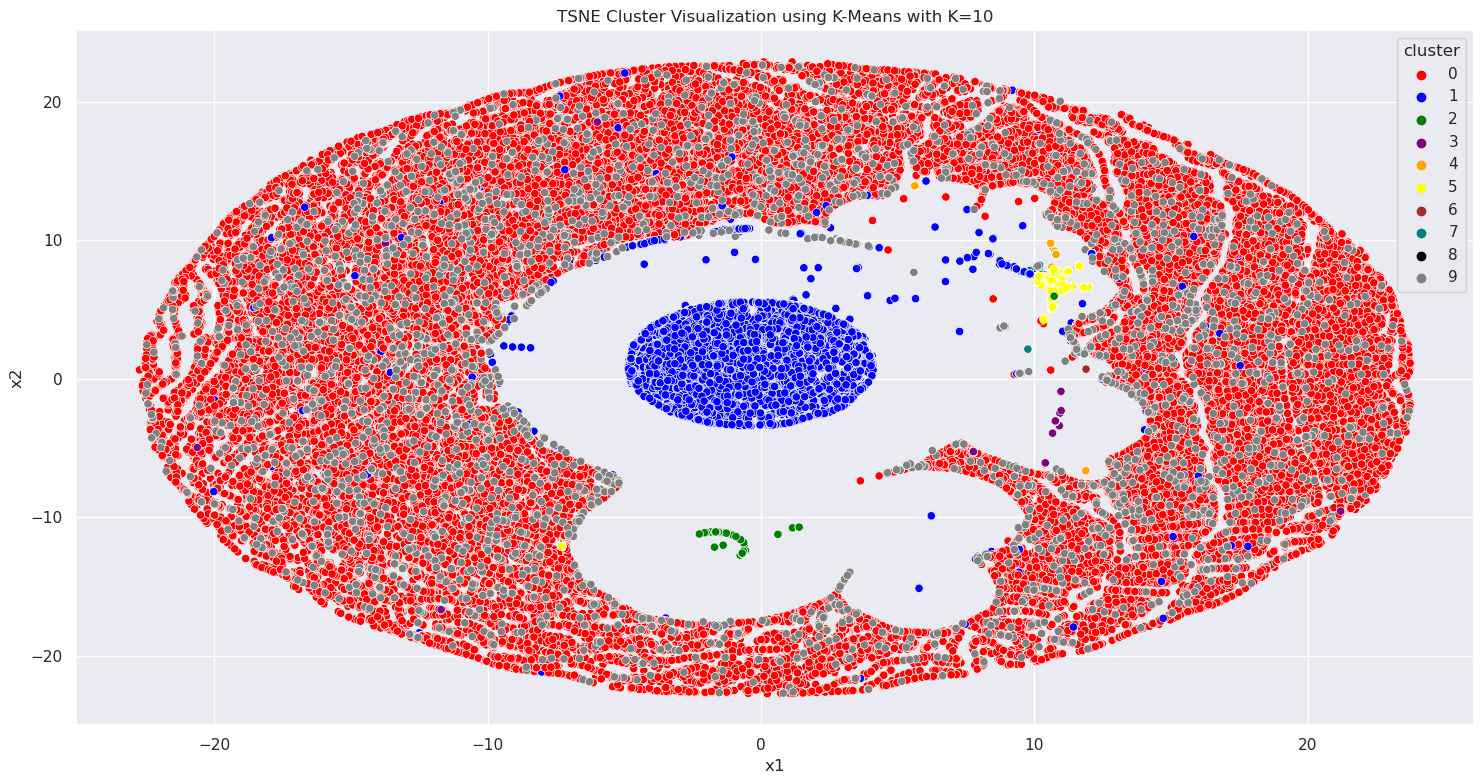
\includegraphics[width=0.8\textwidth]{../figures/plots/section3/tsne_kmeans_clusters.png}
            \caption{t-SNE Visualization of K-Means Clusters}
            \label{fig:tsne-kmeans}
        \end{figure}

        \textbf{Figure \ref{fig:tsne-gmm}} shows the t-SNE visualization of GMM clusters.

        \begin{figure}[h]
            \centering
            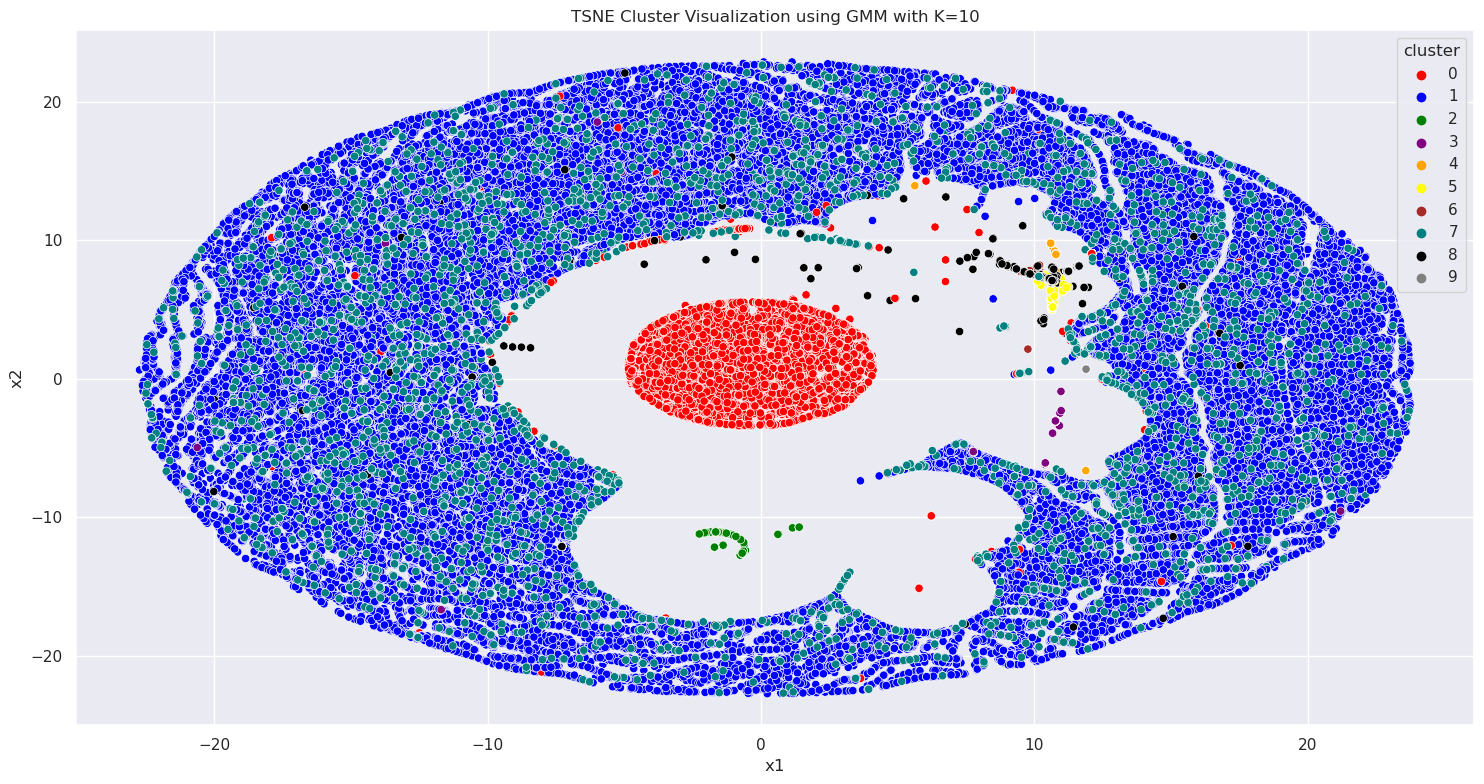
\includegraphics[width=0.8\textwidth]{../figures/plots/section3/tsne_gmm_clusters.png}
            \caption{t-SNE Visualization of GMM Clusters}
            \label{fig:tsne-gmm}
        \end{figure}

    \subsection{Cluster Analysis}
    
        Analyzing the characteristics of each cluster helps in understanding the common patterns and behaviors within the clusters. We examine the distribution of features and intents within each cluster.

        \textbf{Cluster Feature Analysis:}
        
        \vspace{0.5em}

        \textbf{Refer to Appendix \ref{lst:feature_distribution} for the code snippet.}

        The feature distribution analysis revealed that certain clusters have distinct characteristics. For example, Cluster 0 shows a high frequency of certain commands, while Cluster 1 is dominated by different commands. This indicates that the clusters capture different types of attack behaviors.

        \textbf{Figure \ref{fig:cluster-feature-distribution}} shows the feature distribution for Cluster 0.

        \begin{figure}[h]
            \centering
            % \includegraphics[width=0.8\textwidth]{../figures/plots/section3/cluster_0_feature_distribution.png}
            \caption{Feature Distribution for Cluster 0}
            \label{fig:cluster-feature-distribution}
        \end{figure}

    \subsection{Intent Homogeneity}
    
        Assessing if clusters reflect intent division involves examining the homogeneity of intents within each cluster. We calculate the proportion of each intent within the clusters to determine if the clusters are homogeneous.

        \textbf{Intent Homogeneity Analysis:}
        
        \vspace{0.5em}

        \textbf{Refer to Appendix \ref{lst:intent_proportions} for the code snippet.}

        The intent homogeneity analysis revealed that certain clusters are more homogeneous in terms of intents. For example, Cluster 0 has a high proportion of "Discovery" intents, while Cluster 1 has a mix of "Persistence" and "Privilege Escalation" intents.

        \textbf{Figure \ref{fig:intent-proportions}} shows the intent proportions for Cluster 0.

        \begin{figure}[h]
            \centering
            % \includegraphics[width=0.8\textwidth]{../figures/plots/section3/cluster_0_intent_proportions.png}
            \caption{Intent Proportions for Cluster 0}
            \label{fig:intent-proportions}
        \end{figure}
        
    \subsection{Specific Attack Categories}
    
        Associating clusters with specific attack categories involves identifying the common attack patterns within each cluster. We analyze the most frequent attack categories within the clusters to understand their characteristics.

        \textbf{Attack Category Analysis:}
        
        \vspace{0.5em}

        \textbf{Refer to Appendix \ref{lst:attack_categories} for the code snippet.}

        The attack category analysis revealed that certain clusters are associated with specific attack categories. For example, Cluster 0 is dominated by "Brute Force" attacks, while Cluster 1 has a mix of "Credential Access" and "Lateral Movement" attacks.

        \textbf{Figure \ref{fig:attack-categories}} shows the attack categories for Cluster 0.

        \begin{figure}[h]
            \centering
            % \includegraphics[width=0.8\textwidth]{../figures/plots/section3/cluster_0_attack_categories.png}
            \caption{Attack Categories for Cluster 0}
            \label{fig:attack-categories}
        \end{figure}
        